\subsection{\href{https://www.argentina.gob.ar/comision-nacional-de-energia-atomica}{National Atomic Energy Commission}}
   \hypertarget{subsec:cnea}
  I worked at the CNEA as a research fellow in the PET (Positron Emission Tomography) development group.\\
   During the work period, a CNC machine was developed for automatic movement of radioactive material.
   I also code part of the photon coincidence algoritm in VHDL for the FPGA  shown in the figure \ref{fig:cnea1}.\\
   Then I developed the software for acquisition and analysis of raw data from the equipment shown in the figure \ref{fig:cnea2}.
   \begin{figure}
      \begin{center}
         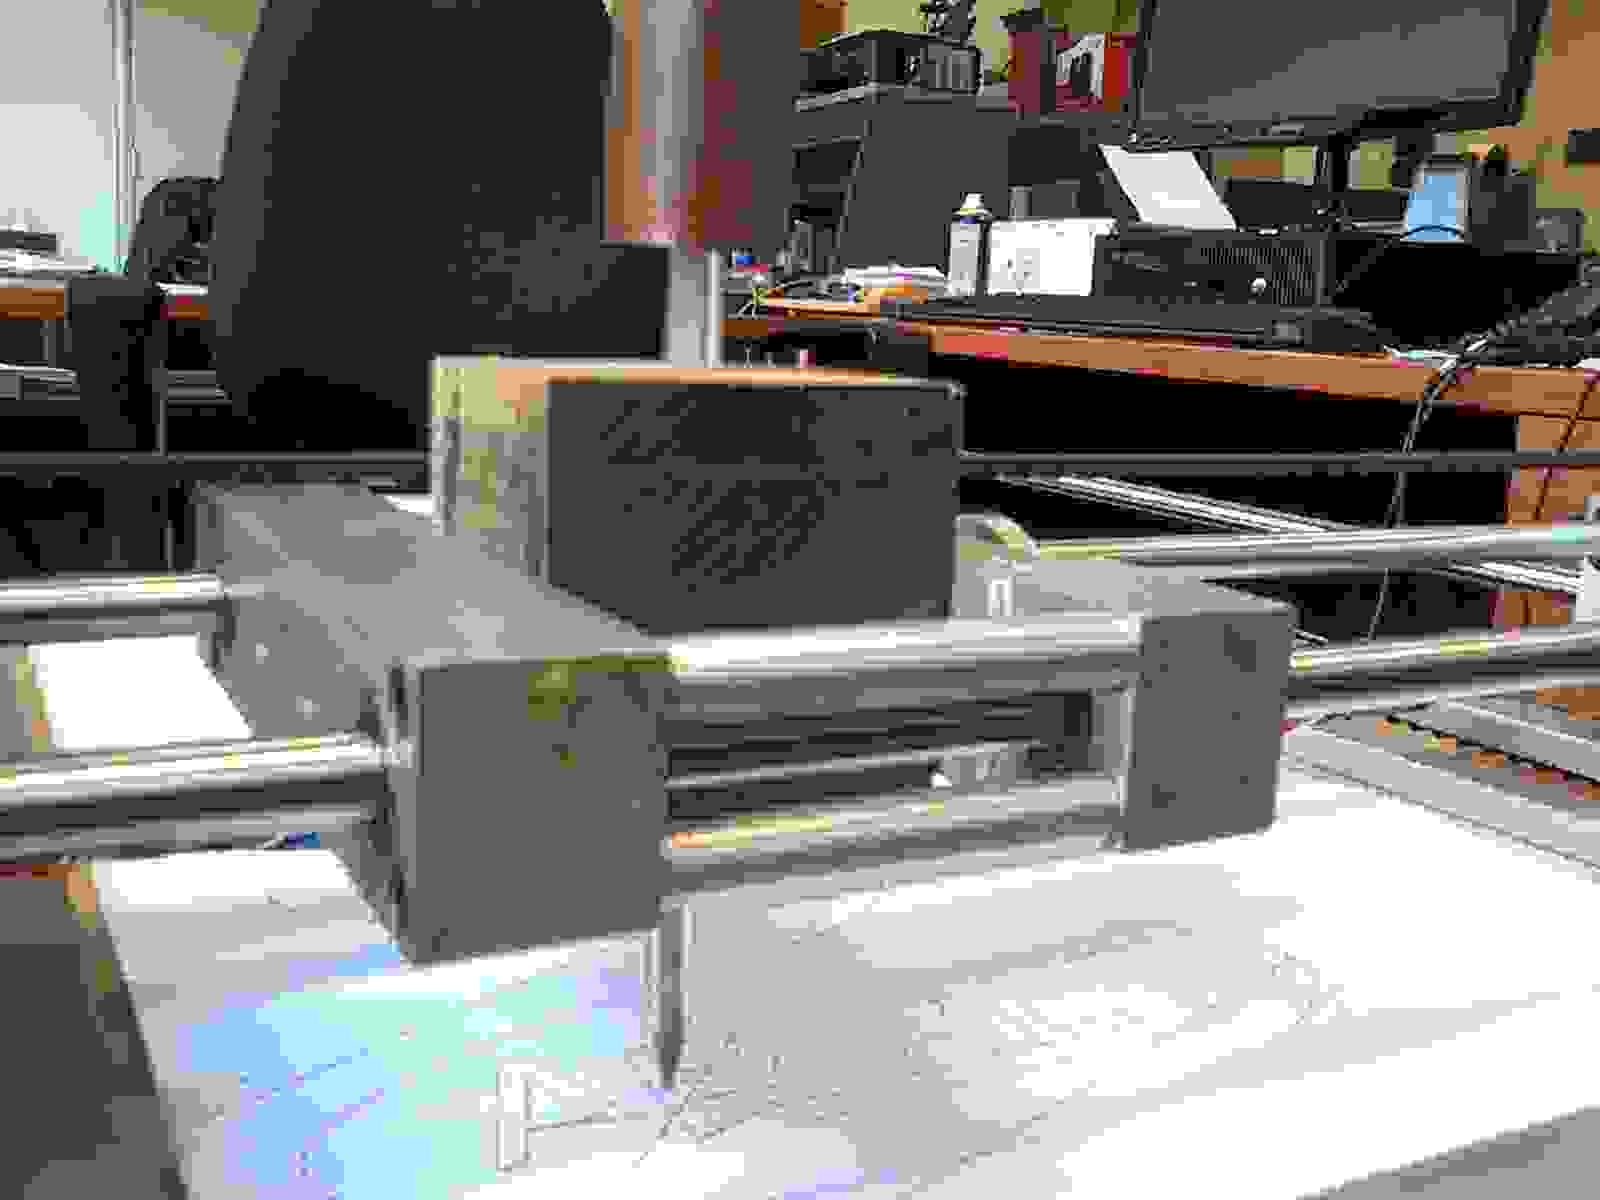
\includegraphics[width=0.24\textwidth]{portfolio/cnea_mesa1.jpg}
         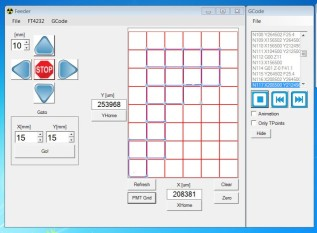
\includegraphics[width=0.24\textwidth]{portfolio/cnea_mesa2.jpg}
         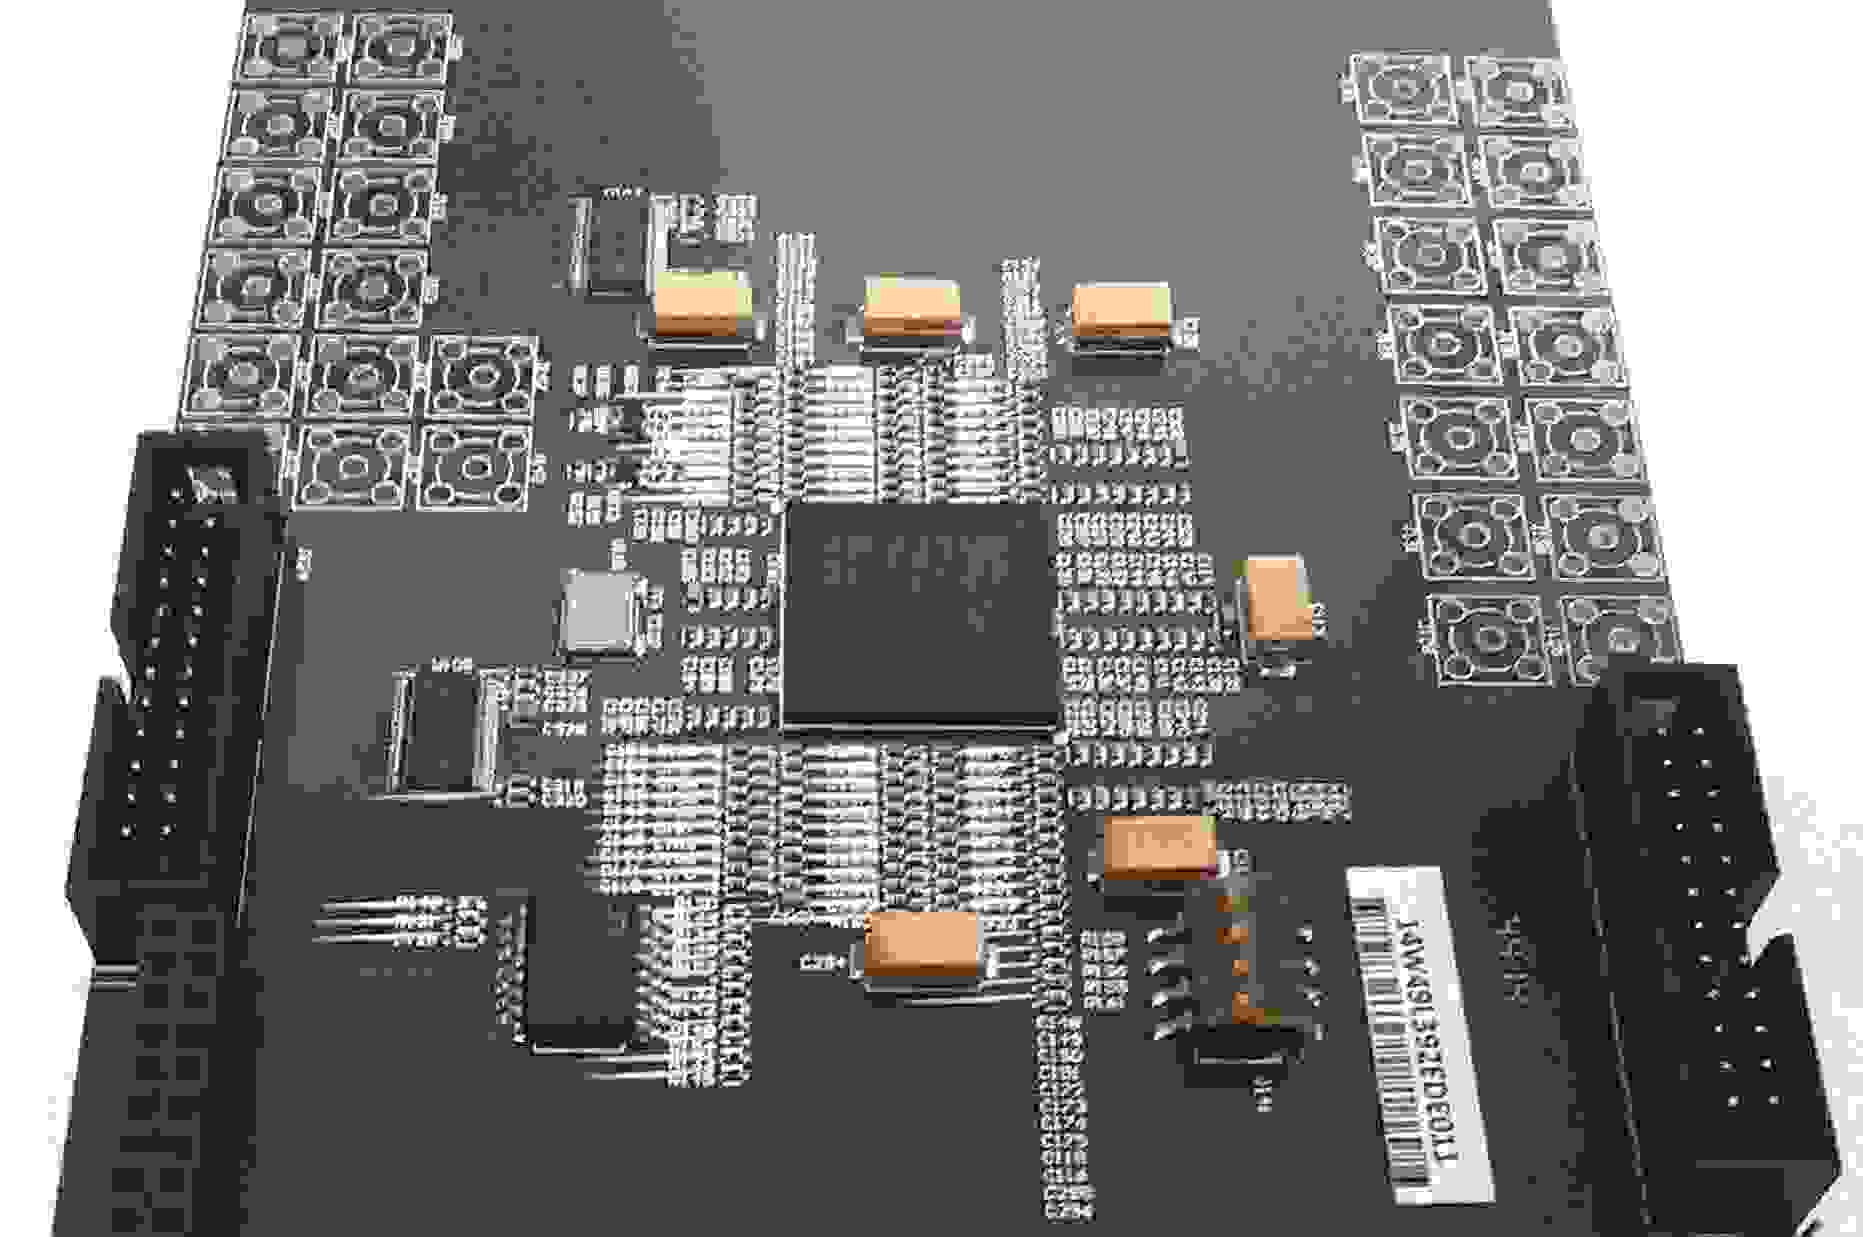
\includegraphics[width=0.24\textwidth]{portfolio/cnea_coin1.jpg}
         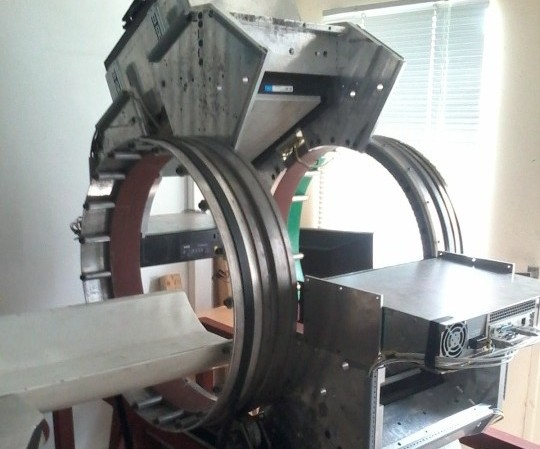
\includegraphics[width=0.24\textwidth]{portfolio/cnea_coin2.jpg}
      \end{center}
      \caption{CNC table for automation of acquisitions with a capture of the management software, the board with the FPGA mounted in one of the 6 heads, and the half-finished tomograph.}
      \label{fig:cnea1}
   \end{figure}
   \begin{figure}
      \begin{center}
         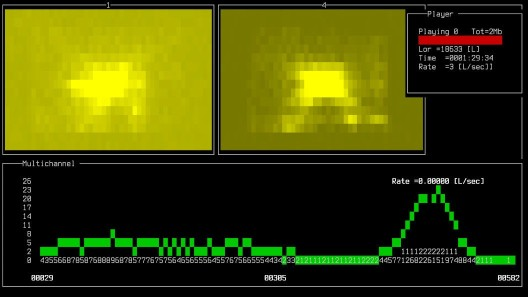
\includegraphics[width=0.24\textwidth]{portfolio/cnea_cuipet1.jpg}
         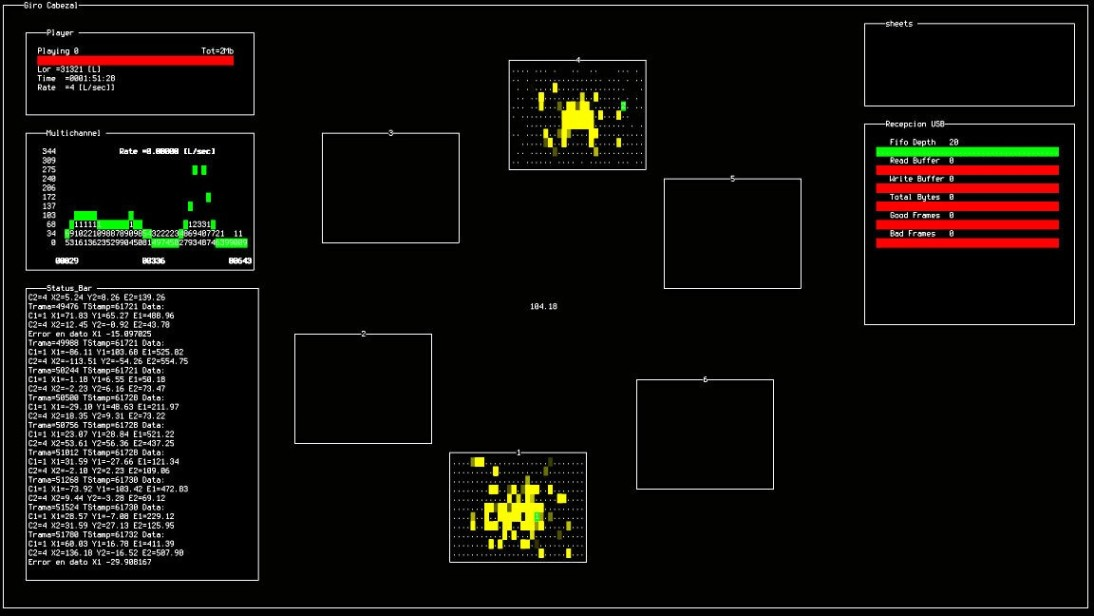
\includegraphics[width=0.24\textwidth]{portfolio/cnea_cuipet5.jpg}
         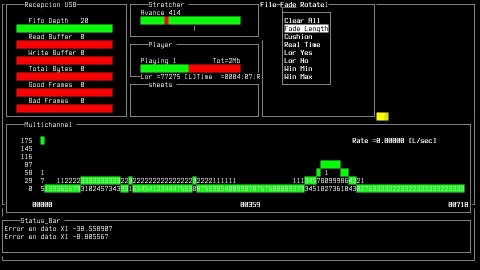
\includegraphics[width=0.24\textwidth]{portfolio/cnea_cuipet3.jpg}
         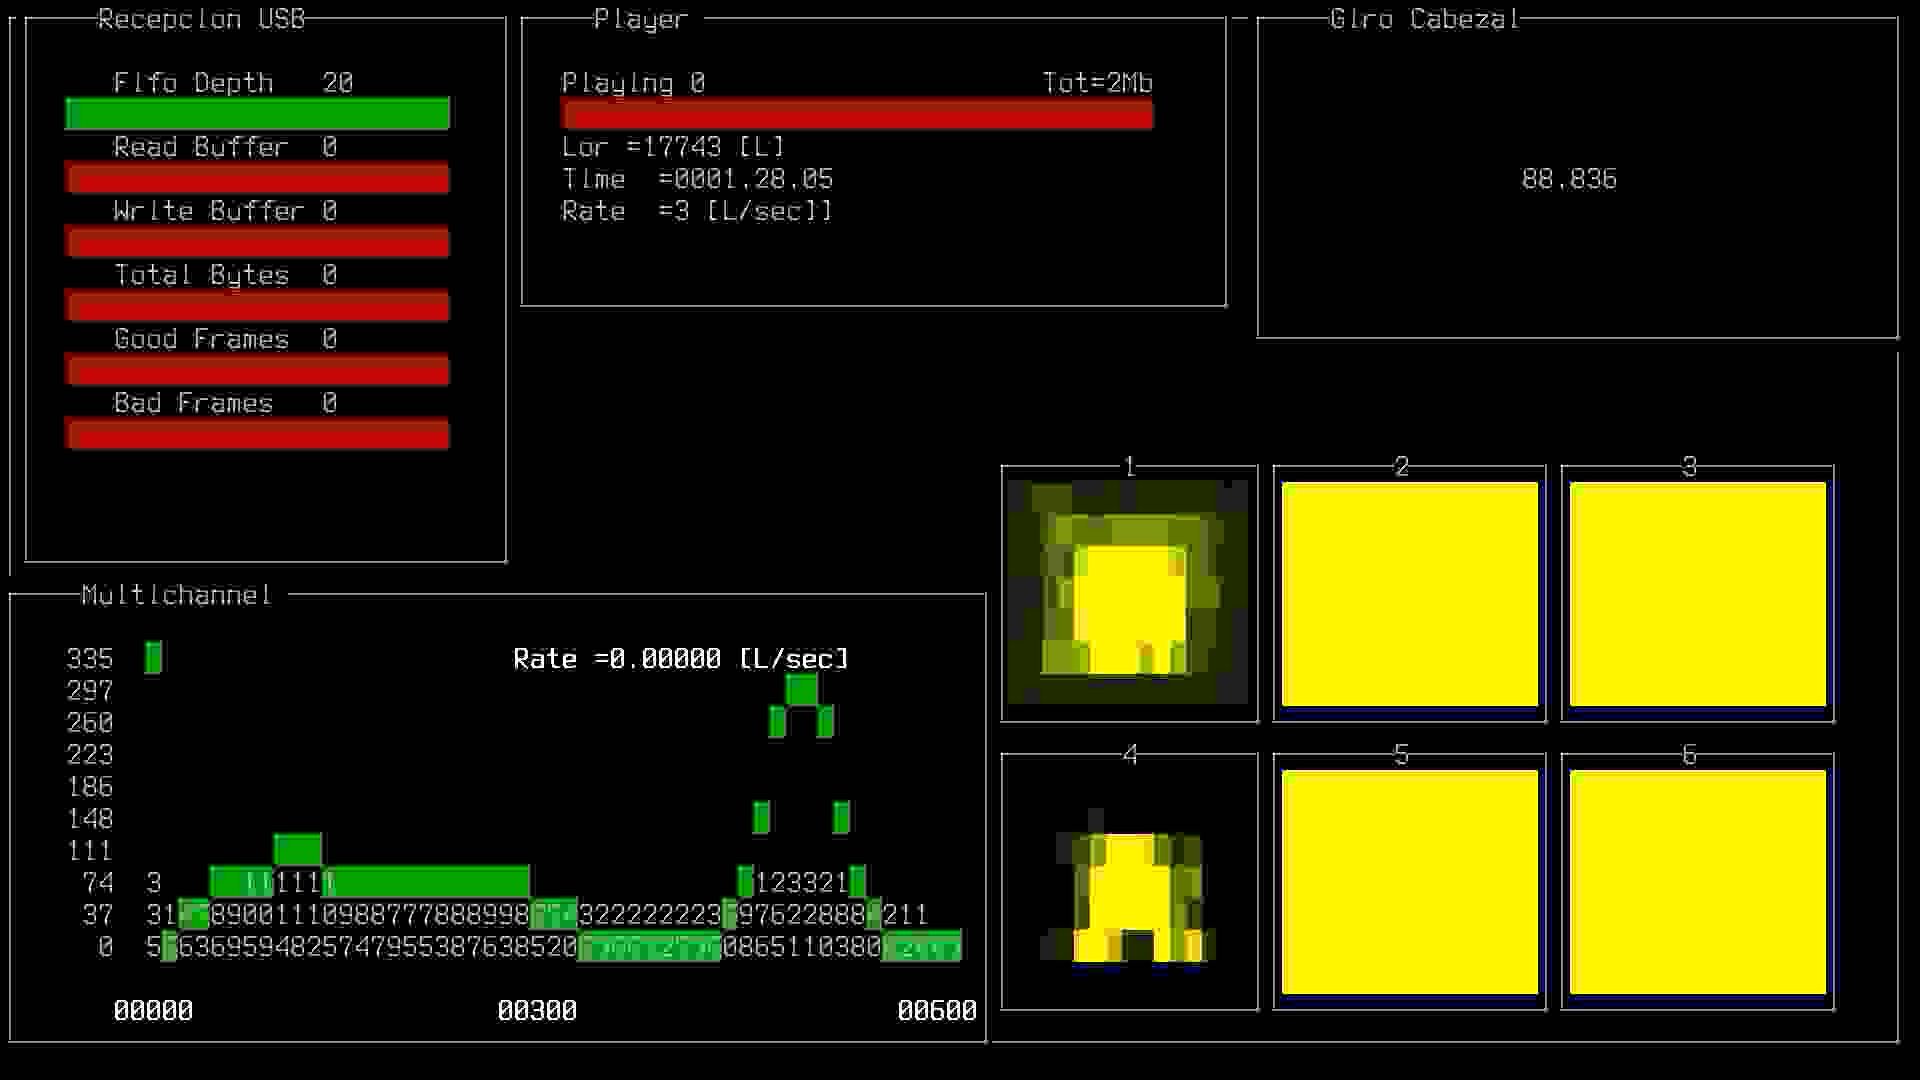
\includegraphics[width=0.24\textwidth]{portfolio/cnea_cuipet4.jpg}
      \end{center}
      \caption{Captures of acquisition software, CUIPET, of the PET at CNEA's lab.}
      \label{fig:cnea2}
   \end{figure}
